% !TeX root = ../main.tex
% !TeX program = xelatex
% !TeX encoding = UTF-8
\section{对照实验与机制分析}
各组分别检验完整场景的连续运行及关键机制，比较对象与固定条件如下。
\subsection{完整服务年与声明冬季回放}

武汉四楼数学场景采用合成的热工与得热参数，四楼分别连接两区域热源，共用系统配电接入。代表时段规划后固定投资，分别回放8784小时服务年和2928小时声明冬季，约束逐楼室温、热源出力、冷热互斥及共享容量。全年还约束地源取排热比例。表\ref{tab:continuous-scope}汇总既有记录，初末室温均为20~$^\circ$C；建筑检查包括每小时末舒适、末态及同小时冷热互斥。

\begin{table}[htbp]
\centering
\caption{四楼场景的连续时序检查}\label{tab:continuous-scope}
\begin{tabularx}{\textwidth}{@{}Xrrr@{}}
\toprule
回放范围 & 连续小时 & 求解gap/\% & 建筑检查违约数\\
\midrule
完整服务年 & 8784 & 0.1344 & 0\\
完整声明冬季 & 2928 & 0.4755 & 0\\
\bottomrule
\end{tabularx}
\end{table}

独立建筑复算的最大RC残差分别为$1.10\times10^{-13}$与$6.75\times10^{-14}$~$^\circ$C，逐时交付保留建筑、区域和原型系统的对应关系。结果支持给定合成参数下的连续运行可行性；该案例选定独立储热及联络管容量均为零，相关模块的机制另按通用模型和独立对照讨论。

\subsection{守恒约束下的负荷分布校正}

六栋外部计量建筑各固定8--10个代表日，仅调整所代表的天数。软校正允许总能量偏差，最小化归一能量残差与权重偏移的组合目标，正则系数固定为$10^{-4}$；硬约束方案要求总能量相等，并直接最小化一阶Wasserstein距离。两者共用总日数和权重下界。归一分布误差为该距离除以该楼保留完整日序列的平均负荷，越小表示负荷大小及出现比例越接近原序列。表\ref{tab:w1}误差均取校正候选；候选失败时回退至原频数权重，另行验收。完整统计准入按能量、分布、峰值和爬坡规则检查最终结果，中位数仅描述这六例。

\begin{figure}[htbp]
\centering
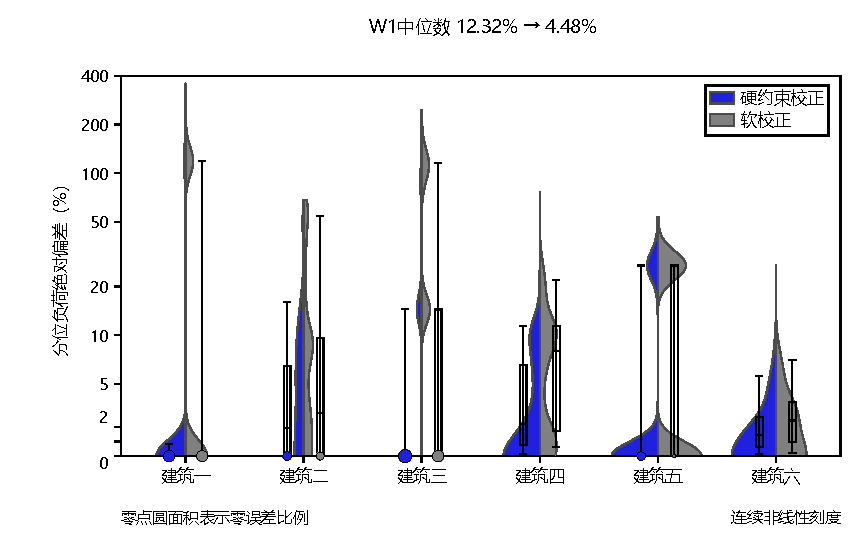
\includegraphics[width=\linewidth]{paper_r2/external_w1.pdf}
\caption{六建筑固定代表日的分布校正。蓝、灰分别表示硬约束与软校正；箱线为加权分位，零点圆面积为零偏差比例。纵轴采用连续非线性刻度，保留完整尾部。}
\label{fig:w1-distribution}
\end{figure}

图\ref{fig:w1-distribution}比较相同累计概率处的原始与代表负荷，展示归一绝对偏差的分布；它反映负荷分布差异，并非逐时预测误差。箱体为25/50/75分位，须为5/95分位，均按原离散概率质量计算。概率加权平均偏差等于对应归一$W_1$；小提琴轮廓仅展示密度。

\begin{table}[htbp]
\centering
\caption{固定代表日集合的权重校正结果}\label{tab:w1}
\begin{tabularx}{\textwidth}{@{}lrrX@{}}
\toprule
建筑 & 软校正误差/\% & 硬约束误差/\% & 硬约束候选的完整准入\\
\midrule
一 & 18.0043 & 4.8097 & 通过\\
二 & 10.0363 & 4.9463 & 原始峰值覆盖不足\\
三 & 20.9090 & 4.1453 & 新增通过\\
四 & 8.2519 & 3.8920 & 通过\\
五 & 14.5937 & 5.4303 & 原始峰值覆盖不足\\
六 & 2.7885 & 2.0065 & 通过\\
\midrule
中位数 & 12.3150 & 4.4775 & 通过数量由3/6增至4/6\\
\bottomrule
\end{tabularx}
\end{table}

六例候选分布误差均下降，中位数由12.3150\%降至4.4775\%，完整统计准入由3/6增至4/6。总能量等式消除加权能量偏差，$W_1$目标调整各负荷水平的出现比例；建筑三因此新增通过。建筑二、五仍因原始峰值覆盖不足被拒绝：调整权重无法补回未保留的峰值。统计准入只检验压缩输入的质量，工程运行可行性仍须通过连续回放校核。

另在已见三城、每城九条固定策略的开发确认中，比较六种权重方法与四档预算。27条连续轨迹共77760小时。硬$W_1$的费用平均绝对百分比误差为0.1405\%，频数法为0.5569\%；实际预算合格选择由9/12增至12/12。其他三种硬方法也达到12/12；这一结果说明压缩质量可以改善固定策略库内的选择，不代表库外全局最优。


\subsection{厂家性能域下的固定设备调度}

TCAV035BHE与TCAV065BHE分别有83、82个Q/P工况点，保留15个缺失角点；同型号有效单元内分别插值制热量Q与输入功率P，再求COP，缺角、越界及跨型号查询均拒绝。在960~m$^2$合成原型上，每城每型号固定一台整机，并固定90~kW电阻补热、80~kW独立制冷和100~kW接入容量。温控基准按当前室温和当小时气象逐时维持舒适范围；LP利用全窗口已给定天气、电价预先安排运行，最小化电量费。六组均覆盖连续2880小时，共用上述资产、20--27~$^\circ$C舒适范围及初末20~$^\circ$C状态。

\begin{table}[htbp]
\centering
\caption{同资产LP相对温控策略的条件运行收益}\label{tab:heatpump}
\begin{tabularx}{\textwidth}{@{}lXrrr@{}}
\toprule
城市 & 型号 & 降费/\% & 节省电量费/元 & 增加电量/kWh\\
\midrule
乌鲁木齐 & TCAV035BHE & 1.3274 & 798.75 & 1398.80\\
乌鲁木齐 & TCAV065BHE & 1.1088 & 474.44 & 753.51\\
固原 & TCAV035BHE & 1.4526 & 908.06 & 1548.64\\
固原 & TCAV065BHE & 1.1013 & 491.80 & 874.83\\
武汉 & TCAV035BHE & 1.1268 & 173.35 & 364.93\\
武汉 & TCAV065BHE & 1.5970 & 237.79 & 728.99\\
\bottomrule
\end{tabularx}
\end{table}

六例电量费降低1.1013\%--1.5970\%，LP目标值与对偶界已按相应编码模型核验。LP在低价时段提前供热，使室温在舒适范围内升高，随后减少高价时段供热；Q/P有效域约束各时段的供热能力与耗电，理想小时占空比表达部分负荷。表\ref{tab:heatpump}所列电量均增加，固定平均因子碳排也随之增加。

\subsection{热容与区域配电约束的交互}

为识别建筑自身的蓄热作用，关闭独立储热，保留两个建筑的温度状态。建筑A固定$H=0.1043$~kW/K、$C=0.535576$~kWh/K；建筑B（图中乙建筑）固定$H=0.15645$~kW/K，仅将$C$从0.535576改为2.142304~kWh/K。另一实验轴为是否施加6.4796375~kW的两楼合计用电上限。四案使用同一武汉气象、2880小时、既有理想设备、20--27~$^\circ$C舒适范围及初末20~$^\circ$C状态；这是热容参数对照，未计现场改造投资。

\begin{table}[htbp]
\centering
\caption{热容倍率与公用电上限的二维对照}\label{tab:factorial}
\begin{tabularx}{\textwidth}{@{}Xrrrr@{}}
\toprule
研究设置 & 电量费/元 & 用电/kWh & 峰值/kW & 绑定小时\\
\midrule
原热容，无公用上限 & 5918.14 & 8155.11 & 14.1064 & ---\\
四倍热容，无公用上限 & 5490.94 & 8725.44 & 25.3335 & ---\\
原热容，有公用上限 & 5937.64 & 8050.61 & 6.4796 & 125\\
四倍热容，有公用上限 & 5660.96 & 8386.07 & 6.4796 & 530\\
\bottomrule
\end{tabularx}
\end{table}

四案均得到求解器容差内最优解，保存的MIP gap为0。共同上限下，增大热容使电量费下降276.68元，即4.6597\%；无共同上限时下降427.20元，即7.2185\%。两项节费之差150.52元，是共同上限削减的热容节费额。共同上限下，区域用电增加335.46~kWh。本组电热设备效率为1，四案无制冷用电且初末温度相同，独立积分核算将该增量分解为建筑A热损减少53.94~kWh、建筑B热损增加389.40~kWh。预热提高室温，也增加向室外散失的热量。

\begin{figure}[htbp]
\centering
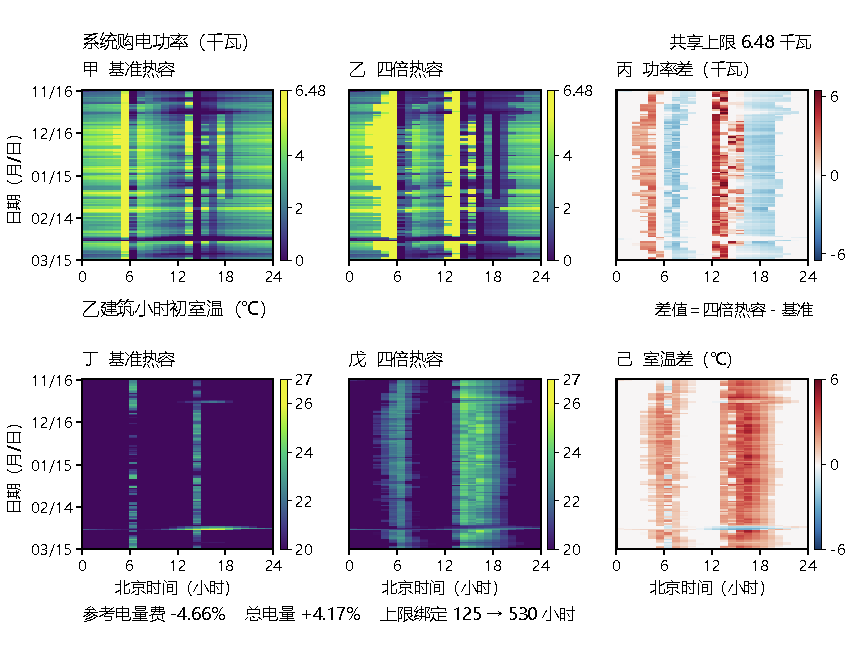
\includegraphics[width=\linewidth]{paper_r2/mechanism_paper/thermal_coupling.pdf}
\caption{共享配电边界下的热惯性调度。上排为系统购电功率，下排为乙建筑小时初室温；第三列为四倍热容减基准。图示完整120日逐时状态，显示预热时移及其容量占用。}
\label{fig:thermal-coupling}
\end{figure}

图\ref{fig:thermal-coupling}将室温变化与购电时移对应起来。绑定小时指两楼合计用电在容差内达到共同上限的小时数，四倍热容使其由125增至530。热容扩大可蓄热空间，也加剧两楼对低价时段容量的竞争，使建筑A的运行与热损随建筑B变化。建筑预热的节费价值因此取决于区域接入容量。

\subsection{管网校核反馈与可行性成本}

在72小时独立泵星型支路参考系统上，固定负荷和设备，在有限稳态模式集合内逐支路检查启用模式的瞬时压降梯度、远端供水温度及逐时热量守恒。将不满足阈值的模式全时段排除后重新优化。表\ref{tab:network}为关闭温差软惩罚的三轮结果，各轮交付热量均为191.5475~kWh。

\begin{table}[htbp]
\centering
\caption{有限网络模式反馈的三轮物理校核结果}\label{tab:network}
\begin{tabularx}{\textwidth}{@{}Xrrr@{}}
\toprule
指标 & 第一轮 & 第二轮 & 第三轮\\
\midrule
最大压降梯度/(Pa/m) & 1081.42 & 504.33 & 237.96\\
最低远端供水温度/$^\circ$C & 61.52 & 59.85 & 57.45\\
管路热损/kWh & 35.70 & 56.94 & 94.44\\
泵耗/kWh & 0.7101 & 0.3570 & 0.1901\\
参考费用/元 & 178.64 & 195.01 & 224.26\\
物理校核 & 压降超限 & 压降超限 & 通过\\
\bottomrule
\end{tabularx}
\end{table}

第三轮满足压降梯度不大于300~Pa/m、远端供水不低于55~$^\circ$C的阈值，得到参考运行费用224.26元的可行方案。排除高流量超限模式后，泵耗与压降下降；较低流量使沿程降温增大、输送同等热量所需启用时间增加，热损与源需求随之上升，费用较第一轮增加25.54\%。反馈给出温压达标的方案及费用代价。第三轮缺少可核验求解下界，所报费用仅作为可行值。

\subsection{三城费用—碳排取舍}

三城另用固定理想资产小原型，以同一温控反馈策略为基准，保持各城天气、舒适和初末状态。费用端点、碳端点分别使电量费、排放最小，中点碳帽取两端排放的平均值。使用共同条件电价与固定平均排放因子；资产与厂家热泵实验不同。表\ref{tab:tradeoff}的降费率以各城基准电量费为分母，增排率以基准排放为分母；节费额保留率为中点节费额除以费用端点节费额。

\begin{table}[htbp]
\centering
\caption{三城中点碳帽方案的决策取舍}\label{tab:tradeoff}
\begin{tabular*}{\textwidth}{@{\extracolsep{\fill}}lrrrr@{}}
\toprule
城市 & 费用端降费/\% & 中点降费/\% & 中点增排/\% & 节费额保留/\%\\
\midrule
乌鲁木齐 & 1.7012 & 1.3916 & 1.7716 & 81.80\\
固原 & 1.7168 & 1.3892 & 1.7469 & 80.92\\
武汉 & 1.7518 & 1.5668 & 2.2003 & 89.44\\
\bottomrule
\end{tabular*}
\end{table}

\begin{figure}[H]
\centering
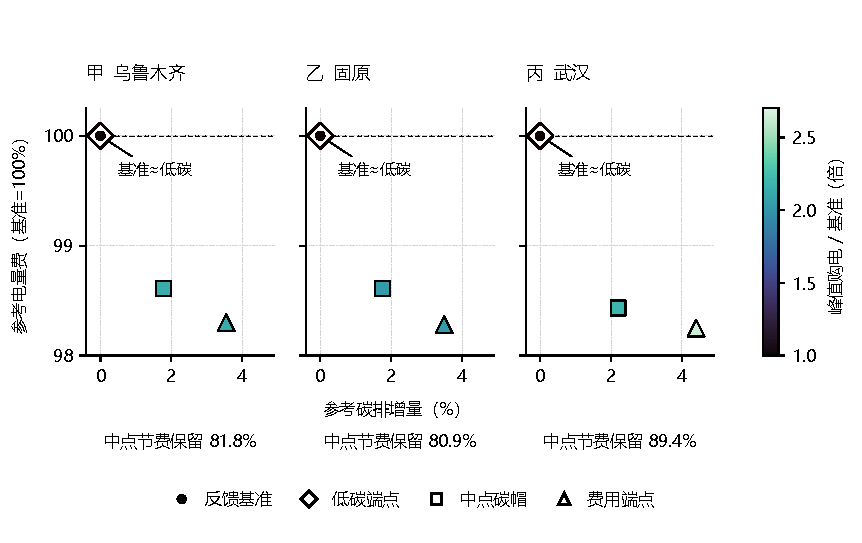
\includegraphics[width=\linewidth]{paper_r2/tradeoff_paper/cost_carbon.pdf}
\caption{三城登记方案的费用、碳排与峰值取舍。图示固定资产实际点，颜色表示峰值与各自基准的比值；中点节费保留率的分母为费用端点相对基准的节省额。}
\label{fig:cost-carbon}
\end{figure}

三城九个优化记录均正常终止，gap不高于$2.63\times10^{-15}$，原运行环境中单记录总耗时3.26--15.27秒。优化点为固定资产问题的容差内最优调度。中点碳帽将费用端点相对基准的增排约减半，同时保留80.92\%--89.44\%的节费额；相对基准仍增排1.75\%--2.20\%。固定平均因子下，碳帽通过限制额外用电，减少可用于低价预热的电量。图\ref{fig:cost-carbon}显示中点峰值仍为基准的2.04--2.21倍，因而排放预算与配电容量需共同考虑。
